\documentclass[
  manuscript=proceedings,  %% article (default), rescience, data, software, proceedings, poster
  layout=preprint,  %% preprint (for submission) or publish (for publisher only)
  year=2026,
  volume=x,
]{extra/joas}
\usepackage{subcaption}
\usepackage{pifont}
\usepackage{makecell}
\usetikzlibrary{positioning,arrows.meta,fit,calc}
\newcommand{\myrowcolour}{\rowcolor[gray]{0.94}}
% \doi{xx.xxxxx/joas.xxxx.xxxx}

% \conference{} command is only used for proceedings
\conference{The 14th OpenSky Symposium}

% \received {1 April 20xx}
% \revised  {1 May 20xx}
% \accepted {10 May 20xx}
% \published{20 May 20xx}

% \editor{Editor Name}

% \reviewers{First Reviewer, Second Reviewer, Third Reviewer}

% specify the .bib file for references
\addbibresource{reference.bib}

% renders in red: anything still awaiting the full-dataset run
\newcommand{\pending}[1]{\textcolor{red}{[#1]}}


% --- below is the area for authors ---

% Title within 12 words
\title{Estimating Aircraft Mass at Top of Descent from ADS-B Trajectory Data}

\author{Aidana Tassanbi \orcid{0009-0009-6286-4713}}
\affiliation{Delft University of Technology, Netherlands}
\email{a.tassanbi@tudelft.nl}

\author{Junzi Sun\orcid{0000-0003-3888-1192}}
\affiliation{Delft University of Technology, Netherlands}

% \author{Jacco Hoekstra\orcid{0000-0002-2734-2719}}
% \affiliation{Delft University of Technology, Netherlands}


% maximum five keywords
\keywords{Aircraft Mass Estimation; Top of Descent; Arrivals; ADS-B; Post-flight Analysis; Machine Learning}

% Important: don't overuse abbreviations. Only use abbreviations if the term is used more than ten times throughout the paper. Otherwise, write them in full.
\abbreviations{
    ADS-B: Automatic Dependent Surveillance–Broadcast,
    MAPE: Mean Absolute Percentage Error,
    MTOW: Maximum Takeoff Weight,
    OEW: Operating Empty Weight,
    RMSE: Root Mean Squared Error,
    TOD: Top of Descent,
    TOW: Takeoff Weight,
    WTC: Wake Turbulence Category
}


\begin{document}
\begin{abstract}
  Aircraft mass strongly affects data-driven flight performance analyses, yet it is generally unavailable in open datasets. For post-flight analyses of arrival trajectories, the relevant quantity is the mass at the top of descent. This work presents a reusable machine learning approach for estimating it from ADS-B data, developed on the EUROCONTROL PRC Data Challenge 2024 dataset, whose disclosed takeoff weights, propagated along each trajectory with the OpenAP fuel flow model, provide reference masses for some 465{,}000 flights. The approach relies only on quantities a researcher can obtain independently: the trajectory itself, the aircraft type from the registry, and openly published aircraft properties. The ADS-B-only model reaches a mean absolute percentage error of 3.39~\% and a root mean squared error of 3{,}638~kg against the reference masses; adding openly available weather and flight information reduces these to 2.55~\% and 2{,}754~kg. The estimate is also robust to incomplete recordings, losing 0.38 percentage points under the coverage gaps measured in real trajectories. We release the pipeline that turns raw OpenSky data into top of descent mass estimates.
\end{abstract}

\section{Introduction}

Aircraft mass is one of the most influential parameters in trajectory prediction, yet it is rarely available in openly accessible datasets. During descent, mass affects the rate of descent and the relationship between speed and altitude from the top of descent (TOD) to the final approach fix. Studies of continuous descent operations~\cite{clarke2004cda,fricke2015cdo}, arrival management~\cite{bronsvoort2013impact}, fuel burn~\cite{lemetti2023arrival}, and noise~\cite{zammit2013accuracy} therefore require an estimate of aircraft mass. A common approach is to assume a fixed fraction of the maximum takeoff weight (MTOW), or 85~\% of the maximum landing weight~\cite{holzapfel2023landing}. While convenient, such assumptions are approximate, and errors in the assumed mass propagate into the predicted trajectory.

Mass estimation from surveillance data has mostly focused on the takeoff and climb phases. Physical approaches fit point-mass or total-energy models to the observed motion, for example to the runway acceleration~\cite{sun2016runway} or to the energy rate in climb~\cite{alligier2013learning,schultz2012adaptive}, or estimate the mass jointly with the thrust setting~\cite{matsuda2026climb}. Others combine several flight phases with Bayesian inference, reaching a mean absolute error of 4.3~\%~\cite{sun2018bayesian}, or track the mass through the flight with a particle filter~\cite{sun2019particle}. Machine learning has been compared with physical estimation for climb prediction~\cite{alligier2015machine} and used to predict distributions of mass and speed rather than single values~\cite{alligier2020predictive}.

When reference masses are available for training, data-driven models reach higher accuracy: 3.6~\% with Gaussian process regression on the takeoff roll~\cite{chati2018gaussian}, 1.48~\% with tree ensembles over several flight phases~\cite{ayzit2023generalizable}, below 3~\% with CNN-LSTM models~\cite{daga2024cnnlstm}, and 2.78~\% with hybrid machine-learning and Bayesian approaches~\cite{wang2025kmidnnbi}. These rely on proprietary flight data, however, which limits their reproducibility and often ties them to a particular operator or fleet.

Fewer studies have addressed mass estimation during descent. Fricke et al.\ inferred mass from approach groundspeed to determine the optimum rate of descent for continuous descents, reporting an average deviation of 12.3~\% over twelve flights~\cite{fricke2015cdo}. Holzäpfel and Rotshteyn inverted the BADA relation between descent speed and mass using Mode S airspeeds and validated the method against 3{,}328 airline-supplied landing weights at Vienna~\cite{holzapfel2023landing}. Salgueiro et al.\ modelled flight management system behaviour and achieved an error of 2.65~\% of MTOW on 240 A320 flights~\cite{salgueiro2025weight}, while Homola et al.\ used stabilised airspeed segments from ADS-B data and reported errors of 6.0--7.0~\% for arrivals of three narrow-body aircraft types~\cite{homola2025airspeed}. These approaches are physically grounded and interpretable, but their validation has generally been limited to a small number of aircraft types from a single airline or airport.

A major obstacle to broader data-driven mass estimation has been the scarcity of reference mass data. The PRC Data Challenge 2024~\cite{prc2024} addressed this limitation by providing disclosed takeoff weights for more than half a million flights with corresponding ADS-B trajectories~\cite{schafer2014bringing}. The best submissions reached errors below 2~\%, for example 1.73~\% with a combination of gradient boosting and neural networks~\cite{murca2025open}. These models are not straightforward to reproduce, however: they require large feature sets and substantial preprocessing, while the highest-performing approaches rely on anonymised airline and operator identifiers that are specific to the challenge dataset. Furthermore, takeoff weight is not equivalent to descent mass, leaving a gap in the availability of open reference data for descent applications.

In this work, we present a model for retrospectively estimating aircraft mass at TOD from ADS-B data, targeting post-flight analysis rather than real-time applications. We use the PRC challenge data as a source of reference labels rather than as a benchmark, and deliberately trade some predictive accuracy for reproducibility by restricting the model inputs to openly available data and excluding challenge-specific or proprietary features. The contributions of this paper are:

\begin{itemize}
\item a reference TOD mass for 464{,}633 flights, obtained by propagating the disclosed takeoff weight using the OpenAP fuel-flow model;
\item gradient boosting models based on four feature sets;
\item a fraction-of-MTOW target formulation and an evaluation of its transferability to aircraft types withheld from training;
\item an assessment of models' sensitivity to incomplete descent coverage;
\item an open pipeline that converts raw OpenSky state vectors into an estimated aircraft mass and is tested on independent arrivals at Amsterdam Airport Schiphol.
\end{itemize}

Section~\ref{sec:method} describes the dataset and presents the reference-mass calculation, features, model, and estimation pipeline; Section~\ref{sec:results} evaluates the four models; Section~\ref{sec:discussion} discusses applicability to unfamiliar aircraft types, incomplete descents, and limitations; and Section~\ref{sec:conclusion} concludes.

\section{Methods}
\label{sec:method}

\begin{figure}
    \centering
    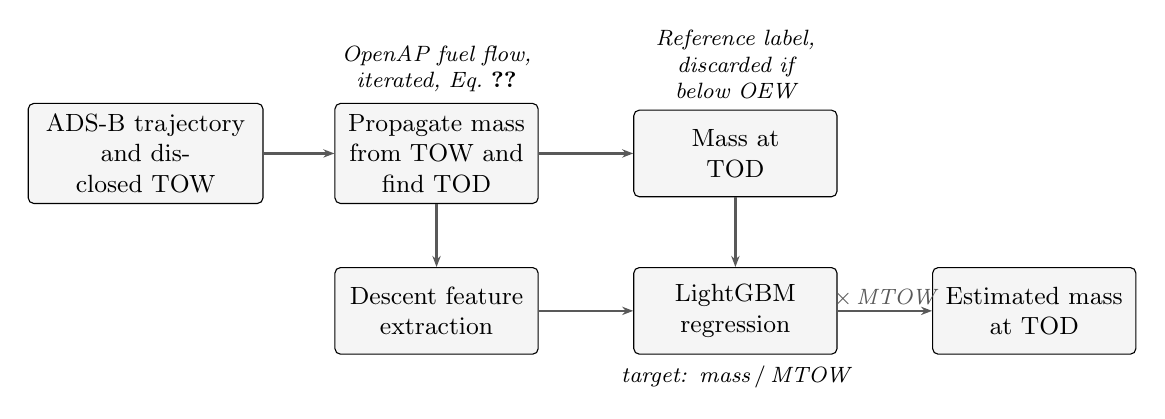
\begin{tikzpicture}[
        font=\small,
        node distance=5mm and 12mm,
        box/.style={
            draw, rounded corners=2pt, align=center,
            inner sep=4pt, minimum height=11mm, text width=23mm,
            fill=black!4
        },
        lab/.style={draw=none, fill=none, text width=30mm, align=center,
                    font=\footnotesize\itshape, inner sep=1pt},
        ar/.style={-{Stealth[length=4pt]}, thick, black!65}
    ]
    %% ---- top row: input, propagation, label ----
    \node[box, text width=27mm] (data) {ADS-B trajectory\\ and disclosed TOW};
    \node[box, right=9mm of data] (prop) {Propagate mass\\ from TOW and\\ find TOD};
    \node[box, right=of prop] (tod) {Mass at\\ TOD};

    \draw[ar] (data) -- (prop);
    \draw[ar] (prop) -- (tod);

    \node[lab, above=1mm of prop] {OpenAP fuel flow,\\ iterated, Eq.~\ref{eqn:ff_from_tow}};
    \node[lab, above=1mm of tod]  {Reference label,\\ discarded if below OEW};

    %% ---- bottom row: features, model, estimate ----
    \node[box, below=8mm of prop] (feat) {Descent feature\\ extraction};
    \node[box, right=of feat]      (regr) {LightGBM\\ regression};
    \node[box, right=of regr]      (mass) {Estimated mass\\ at TOD};

    \draw[ar] (prop) -- (feat);
    \draw[ar] (tod)  -- (regr);
    \draw[ar] (feat) -- (regr);
    \draw[ar] (regr) -- node[above=0.4mm, font=\footnotesize\itshape,
        text=black!65, inner sep=0pt] {$\times$\,MTOW} (mass);

    \node[lab, below=1mm of regr] {target: mass\,$/$\,MTOW};
    \end{tikzpicture}
    \caption{Workflow for the modelling and estimation process. The disclosed TOW is propagated along the trajectory to give a reference mass at TOD, which is subject to a physical check, and a gradient boosting model is trained to recover that mass as a fraction of the MTOW.}
    \label{fig:workflow}
\end{figure}

Training a model to estimate the TOD mass first requires reliable reference values of that mass. None are disclosed, so they are derived by propagating the disclosed TOW along each flight, and the propagation is only as reliable as the trajectory it integrates over: the trajectories must first be reconstructed and cleaned of noise and spikes. The method follows that order, from preprocessing (Section~\ref{sec:preprocessing}) to the reference mass (Section~\ref{sec:label}) and only then to the model. Figure~\ref{fig:workflow} summarises the workflow: the disclosed TOW is propagated along each full flight trajectory to obtain a reference mass at TOD, features are extracted from the descent, and a gradient boosting model is trained to recover that mass.




\subsection{Data}
\label{sec:data}

The models are trained on the EUROCONTROL PRC Data Challenge 2024 dataset~\cite{prc2024}, which covers 527{,}162 European flights across 30 aircraft types over one year. For each flight it provides an ADS-B trajectory, weather variables interpolated at every trajectory point, the actual takeoff weight (TOW), and airport and flight information.

\subsection{Trajectory preprocessing}
\label{sec:preprocessing}

Trajectories are processed with the \texttt{traffic} library~\cite{traffic}. Each flight is first passed through an outlier filter and discarded if it contains fewer than ten samples or if its 80th percentile altitude is below 10{,}000~ft, which removes ground movements and low-level traffic. The remaining trajectories are resampled to a uniform 15~s interval. True airspeed is not broadcast, so it is reconstructed from the groundspeed and the wind, both of which are provided in the dataset. Flight phases are labelled with the phase detection of \texttt{OpenAP} applied using \texttt{traffic}. Because the cruise label alone is noisy for stepped or interrupted cruises, the cruise segment is refined: a sample is retained as cruise only if it lies between the last climb sample and the first descent sample, is labelled cruise or level, sits between 20{,}000 and 45{,}000~ft, and has a vertical rate below 500~ft/min in magnitude. The climb and cruise are used in the mass propagation only. Apart from the state at the last cruise sample, which marks the TOD, no trajectory feature is taken from outside the descent.

\subsection{Reference mass at TOD}
\label{sec:label}

The TOD mass is derived from the takeoff weight and full trajectory. We evaluate the OpenAP fuel flow model~\cite{openap} along each trajectory using the disclosed TOW, true airspeed, altitude, vertical rate, and temperature deviation $\Delta T$ from the standard atmosphere at the lowest flight sample. Subtracting the cumulative fuel burnt from the TOW gives the mass at every sample,

\begin{equation}
    \label{eqn:ff_from_tow}
    m_n = m_0 - \sum_{i=0}^{n} ff_i \cdot \Delta t_i ,
    \qquad \forall n \in \{0, 1, \ldots, k\},
\end{equation}

\noindent where $m_0$ is the TOW, $\Delta t_i$ the interval preceding sample $i$, and $ff_i$ the fuel flow there. Because $ff_i$ itself depends on the mass $m_i$, the profile is solved by fixed-point iteration: all masses start at $m_0$, and each pass re-evaluates the fuel flow at the masses of the previous pass and re-accumulates the sum. The iteration settles within two passes and is run for five. The reference TOD mass is the mass at the first sample of the descent phase. It remains a derived quantity, so any error of the fuel flow model propagates into the training target (Section~\ref{sec:limitations}).


A reference TOD mass is obtained for 480{,}946 flights, 91.2~\% of the release. The losses are due to data limitations. Two types, the BCS1 and BCS3, have no OpenAP performance model, so no mass can be propagated for them. Beyond that, a trajectory must contain an identifiable cruise and descent to be usable, which excludes flights that are too short, too low, or too sparsely covered.

\subsection{Training set}
\label{sec:trainingset}

The labels are screened before training to exclude physically impossible values: 438 flights with disclosed TOW exceeding 105~\% of MTOW, and 15{,}863 flights whose propagated mass at TOD falls below the published operating empty weight (OEW), are discarded. The second group is concentrated in four types of the Boeing 777 and 787 families: 80~\% of the B772 labels, 30~\% of the B77W, 28~\% of the B789 and 18~\% of the B788 fall below the OEW, which suggests that the OpenAP fuel flow over-burns for these types across a long cruise. It is not a property of heavy aircraft in general: the other heavy types, the A332, A333, A343, A359 and B763, lose at most 0.2~\% of their labels, and no medium type more than 0.1~\%. If the OpenAP fuel flow model for these types improves, the released models can be retrained to recover these flights.

The number of flights per aircraft type among the labelled flights is strongly uneven: the A320 alone accounts for 23.2~\% of the flights, while the five rarest aircraft types together contribute 19 flights. Types represented by fewer than 100 labelled flights are excluded, since under a random train--test split such a type is either never tested or tested with no training examples of its own. This leaves 23 aircraft types and 464{,}633 flights, and the train/test split 80/20 gives 371{,}706 and 92{,}927 flights respectively. The split is drawn once and shared by the four models of Section~\ref{sec:results} (also, in the evaluation of one of these models in Section~\ref{sec:missing}), so that comparisons between feature sets are not confounded by it. The experiment on unfamiliar aircraft types in Section~\ref{sec:unseen} uses a different split.

\subsection{Features}
\label{sec:features}

Features are aggregated over the descent, so that the estimate reflects the recorded arrival trajectory. They are combined with quantities describing the aircraft and the arrival, all obtainable outside the dataset: the aircraft type is resolved from the \texttt{icao24} transponder address through the aircraft registry shipped with \texttt{traffic}; the MTOW and OEW are read from OpenAP, with published values substituted for the types OpenAP either lacks or resolves to an unsuitable synonym; and the wake turbulence category (WTC) is derived from that mass using the ICAO thresholds.


Table~\ref{tab:features} lists every feature, grouped by data source that a user needs in order to compute or derive it. The grouping defines four levels of data availability, and their performance is compared in Section~\ref{sec:results}:

\begin{enumerate}
  \item \textbf{ADS-B only} (18 features), using the trajectory together with the open aircraft properties above.
  \item \textbf{ADS-B and weather} ($18+6$ features), adding meteorological variables supplied in the dataset by \texttt{fastmeteo}~\cite{fastmeteo}, which is open and easy to use but requires local storage of the weather data and may take a long time to download the weather grids, depending on the extent of the data and the speed of the connection. Airspeed is not broadcast, so every airspeed-derived feature falls in this group.
  \item \textbf{ADS-B and flight information} ($18+5$ features), adding contextual features such as origin airport location, flight duration, and distance between airports, which are open but must be retrieved separately, for instance from an OpenSky flight list.
  \item \textbf{ADS-B, weather, and flight information} ($18+6+5$ features), using all considered features.
\end{enumerate}

\begin{table}[htbp]
    \centering
    \small
    \begin{tabular}{@{}lp{0.22\linewidth}p{0.55\linewidth}@{}}
    \toprule
    \textbf{Data source} & \textbf{Feature} & \textbf{Description} \\
    \midrule

    \textbf{ADS-B}
        & \texttt{aircraft\_type} & ICAO type designator, from the \texttt{icao24} address \\
    & \texttt{wtc} & WTC, from the ICAO mass thresholds \\
    & \texttt{m\_tow} & Maximum takeoff mass of the type from OpenAP [kg] \\
    & \texttt{oew} & Operating empty weight of the type from OpenAP [kg] \\
    & \texttt{ades} & Arrival airport, ICAO code \\
    & \texttt{lat\_arr}, \texttt{lon\_arr} & Position of the arrival airport [deg] \\
    & \texttt{mean\_rod} & Mean rate of descent [ft/min] \\
    & \texttt{median\_rod} & Median rate of descent [ft/min] \\
    & \texttt{min\_rod} & Steepest rate of descent [ft/min] \\
    & \texttt{dur\_descent} & Duration of the descent phase [s] \\
    & \texttt{des\_gs\_min} & Minimum groundspeed during the descent [kt] \\
    & \texttt{des\_gs\_mean} & Mean groundspeed during the descent [kt] \\
    & \texttt{des\_gs\_max} & Maximum groundspeed during the descent [kt] \\
    & \texttt{tod\_alt} & Altitude at the last cruise sample [ft] \\
    & \texttt{tod\_gs} & Groundspeed at the last cruise sample [kt] \\
    & \texttt{time\_of\_day\_arrival} & Hour of arrival \\
    & \texttt{day\_of\_year} & Day of the year \\[3pt]
\midrule
    \textbf{Weather}
        & \texttt{des\_tas\_min} & Minimum true airspeed during the descent [kt] \\
    & \texttt{des\_tas\_mean} & Mean true airspeed during the descent [kt] \\
    & \texttt{des\_tas\_max} & Maximum true airspeed during the descent [kt] \\
    & \texttt{tod\_tas} & True airspeed at the last cruise sample [kt] \\
    & \texttt{des\_dist} & Air distance flown during the descent [km] \\
    & \texttt{des\_temp} & Highest air temperature during the descent [K] \\[3pt]
\midrule
    \textbf{Flight information}
        & \texttt{adep} & Departure airport, ICAO code \\
    & \texttt{lat\_dep}, \texttt{lon\_dep} & Position of the departure airport [deg] \\
    & \texttt{flight\_duration} & Flight duration [min] \\
    & \texttt{distance\_ap} & Great-circle distance between the airports [m] \\

    \bottomrule
    \end{tabular}
    \caption{List of features used for training.}
    \label{tab:features}
\end{table}

\subsection{Model}

The quantity regressed is not the mass itself but its fraction of the MTOW, the prediction being multiplied back by that mass to return kilograms. This allows the model to scale to aircraft types it was not trained on, and extends its usability.

A single model is trained across the 23 retained aircraft types (the filtering is described in Section~\ref{sec:trainingset}), with aircraft type included as a categorical feature. LightGBM~\cite{lgbm} is chosen for practical reasons, as it is easy to install, handles missing values natively, supports categorical features, and predicts quickly. The categorical features keep their own values, so the trained model carries its category levels and can encode new data without a separate encoder. Prediction is restricted to a single thread so that the model can be evaluated inside the parallel workers of a trajectory processing pipeline.

\subsection{The released pipeline}
\label{sec:released}

Everything above is applied to the challenge dataset, in which the trajectories are already split into identified flights with a known aircraft type. To make the model applicable to other data, the same chain is packaged as a single pipeline from raw OpenSky state vectors to an estimated mass at TOD. It normalises column names and units with \texttt{traffic}, applies the preprocessing of Section~\ref{sec:preprocessing} and the features of Section~\ref{sec:features}, deriving winds from \texttt{fastmeteo} when weather is requested, and discards descents shorter than 345~s as truncated and types with no known MTOW. The arrival airport is inferred from the end of the track unless a flight list supplies it. \ref{app:pipeline} shows that the pipeline reproduces the training features from raw recordings, and reports its behaviour on half a day of arrivals at Amsterdam Schiphol.
\begin{figure}
    \centering
    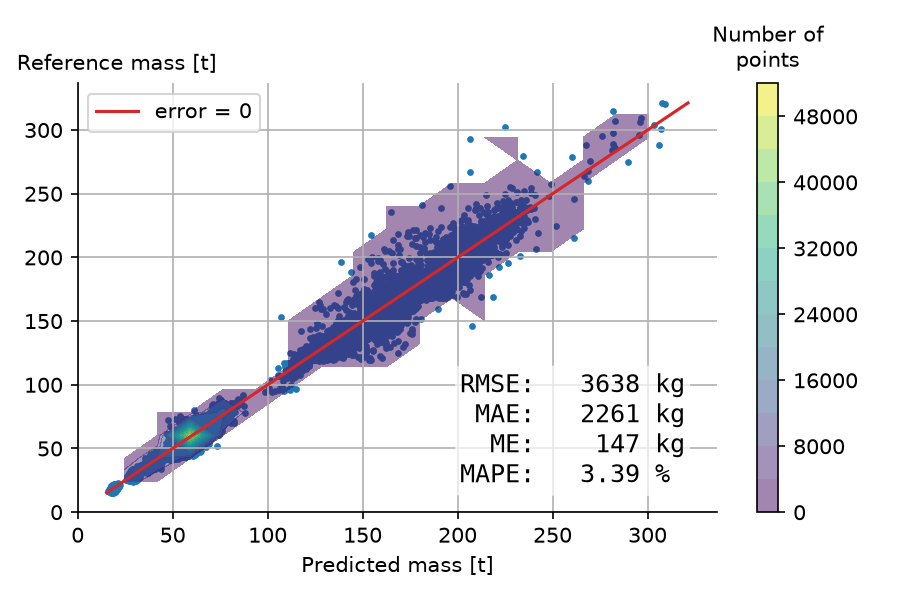
\includegraphics[width=0.7\linewidth]{figures/test_train_tod_noweather_all.png}
    \caption{Estimation errors of the ADS-B-only model on the test set.}
    \label{fig:results}
\end{figure}
\section{Results}
\label{sec:results}

Four models are trained, one on each of the feature sets of Section~\ref{sec:features}. Both metrics are computed on the 20~\% of the dataset that no model sees during training. The mean absolute percentage error (MAPE) and the root mean squared error (RMSE) are defined as follows:

\begin{equation}
    \text{MAPE}
    = \frac{1}{n_{\text{flights}}}
      \sum_{i=1}^{n_{\text{flights}}}
      \frac{\left| m^{(i)}_{\text{ref}} - m^{(i)}_{\text{pred}} \right|}
      {m^{(i)}_{\text{ref}}} \times 100~\%,
    \label{eq:mape}
\end{equation}

\begin{equation}
    \text{RMSE}
    = \sqrt{\frac{1}{ n_{\text{flights}}}\sum_{i=1}^{n_{\text{flights}}} (m_{\text{ref}} - m_{\text{pred}})^2},
    \label{eq:rmse}
\end{equation}

\noindent where $m_{\text{ref}}$ denotes the reference mass at TOD constructed in Section~\ref{sec:label}, $m_{\text{pred}}$ the model estimate, and $n_{\text{flights}}$ the number of flights in the test set.




The ADS-B-only model reaches a MAPE of 3.39~\% and an RMSE of 3{,}638~kg against the derived reference masses in the test set, as illustrated in Figure~\ref{fig:results}. Table~\ref{tab:mapes} reports the performance of the models trained with additional weather and/or flight information. Flight information alone lowers the RMSE by 770~kg, whereas weather alone lowers it by 137~kg; together they reduce it by 884~kg, about a quarter. The origin airport and the distance flown are evidently better proxies for the fuel loaded, and hence for the mass, than the atmospheric conditions encountered during the descent.

\begin{table}[htbp]
    \centering
    \small
    \begin{tabular}{@{}ccc|rr@{}}
    \toprule
    \multicolumn{3}{c|}{\textbf{Features included}} & \multicolumn{2}{c}{\textbf{Test-set error}} \\
    \cmidrule(r){1-3}\cmidrule(l){4-5}
    ADS-B & Weather & Flight information & RMSE [kg] & MAPE [\%] \\
    \midrule
    \ding{51} & \ding{51} & \ding{51} & 2{,}754 & 2.55 \\
    \ding{51} & \ding{51} & \ding{55} & 3{,}501 & 3.15 \\
    \ding{51} & \ding{55} & \ding{51} & 2{,}868 & 2.72 \\
    \ding{51} & \ding{55} & \ding{55} & 3{,}638 & 3.39 \\
    \bottomrule
    \end{tabular}
    \caption{Estimation results on the test set with the four feature sets.}
    \label{tab:mapes}
\end{table}

Table~\ref{tab:pertype} breaks the ADS-B-only model down by aircraft type. The absolute error tracks aircraft size closely, from 1{,}112~kg for the AT76 to 11{,}605~kg for the B772, and the split by WTC is sharp: every heavy type exceeds 5{,}500~kg while every medium type stays below 3{,}300~kg. The heavies therefore dominate the pooled RMSE despite making up a small share of the flights. The relative error is far more uniform, between 1.85~\% and 4.67~\% across all 23 types, which indicates that the model is not simply failing on the rarer types: the A319, with 24{,}649 flights, and the A332, with 3{,}102, reach a comparable MAPE. Figure~\ref{fig:pertype} shows the same breakdown for all four feature sets. The full feature set is the best of the four for 20 of the 23 types, the exceptions being the A319, the B763 and the B772, so the ordering seen in Table~\ref{tab:mapes} is not an artefact of pooling. The largest reductions in error from the additional features are on the A320, the B77W and the B788, which fall by 1.2 to 1.3 percentage points, the B77W from 3.90~\% to 2.66~\%; the two types the ADS-B-only model finds hardest, the B772 at 4.67~\% and the AT76 at 4.66~\%, improve less, by about 0.75. Weather on its own, by contrast, leaves several types essentially unchanged: the E190, the B77W, the B789 and the A332 move by less than 0.06 percentage points.



\begin{figure}
    \centering
    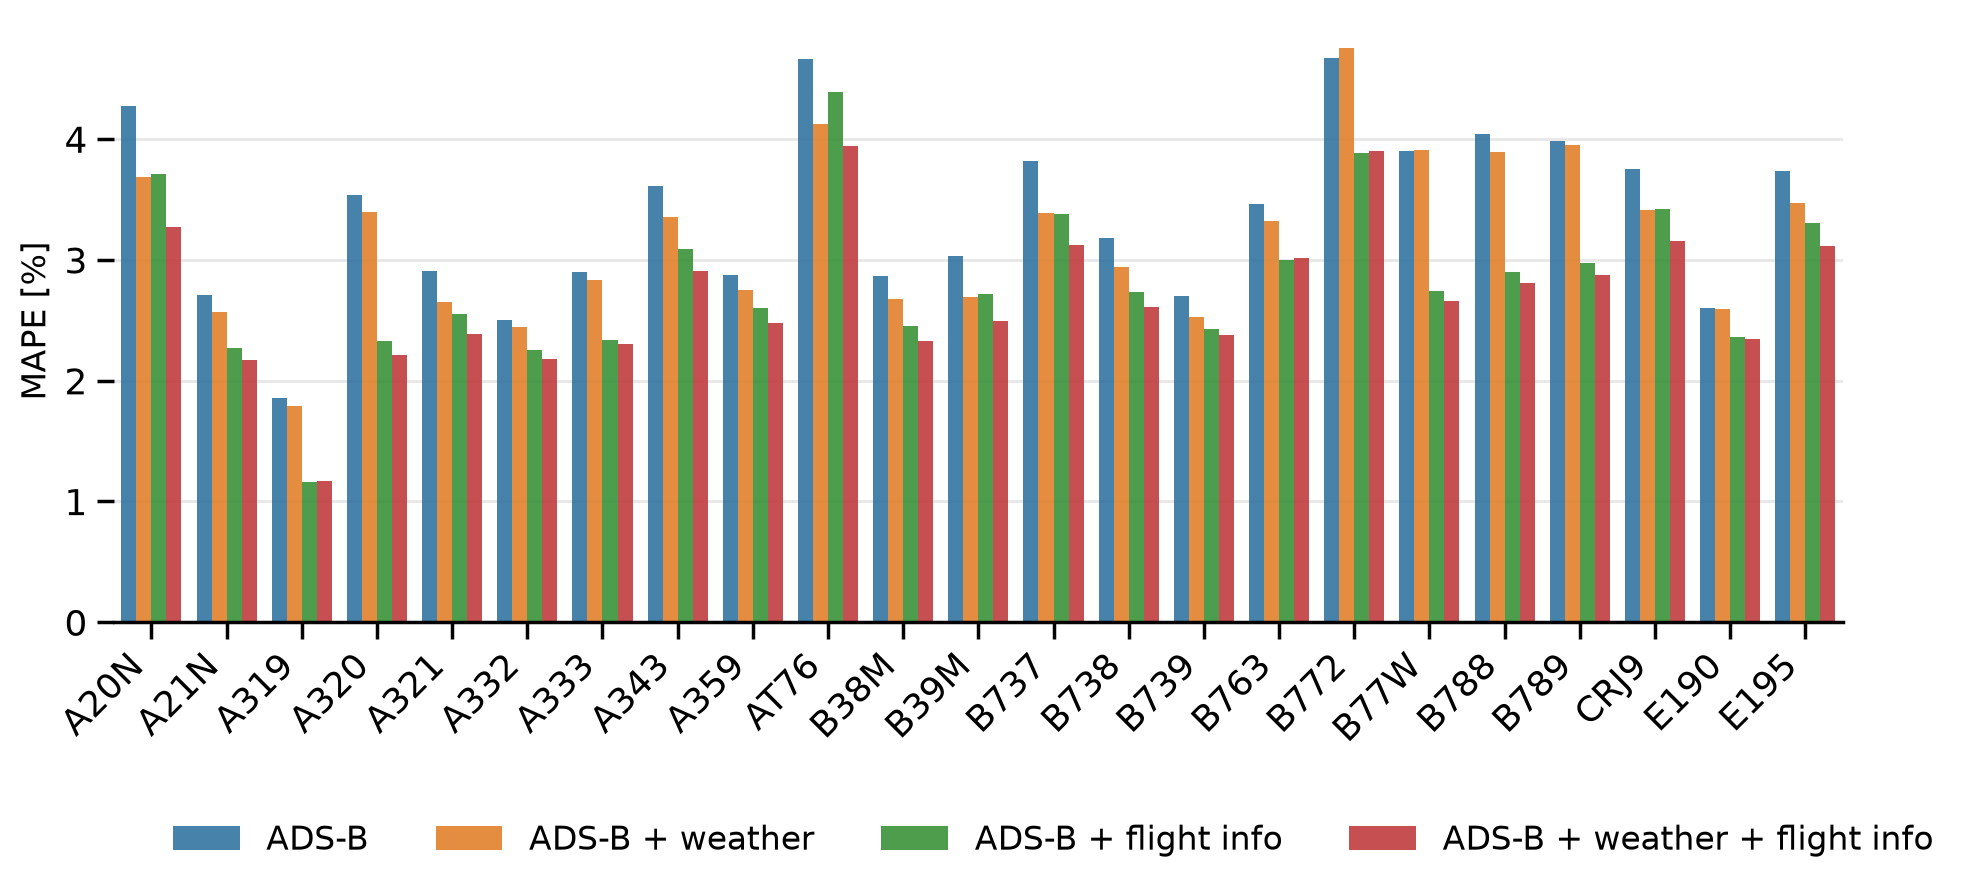
\includegraphics[width=\linewidth]{figures/mape_per_ac.png}
    \caption{Relative error per aircraft type, for each of the four feature sets.}
    \label{fig:pertype}
\end{figure}

\begin{table}[htbp]
    \centering
    \caption{Per-type performance of the ADS-B-only model on the test split.}
    \begin{minipage}[t]{0.48\textwidth}
    \vspace{0pt}
    \centering
    \small
    \setlength{\tabcolsep}{4pt}
    \begin{tabular}{rc|crrrr}
    \toprule
    && & \multicolumn{2}{c}{\textbf{Flights}} & \multicolumn{2}{c}{\textbf{Test-set error}}\\
    \cmidrule(lr){4-5}\cmidrule(lr){6-7}
    & \thead{Aircraft\\type} & \thead{WTC} & \thead{total} & \thead{test} & \thead{RMSE\\{}[kg]} & \thead{MAPE\\{}[\%]} \\
    \midrule
    1 & A20N & M & 52{,}855 & 10{,}479 & 3{,}209 & 4.28 \\
    \myrowcolour
    2 & A21N & M & 31{,}515 & 6{,}230 & 2{,}609 & 2.71 \\
    3 & A319 & M & 24{,}649 & 4{,}948 & 1{,}502 & 1.85 \\
    \myrowcolour
    4 & A320 & M & 111{,}396 & 22{,}227 & 2{,}847 & 3.54 \\
    5 & A321 & M & 39{,}890 & 7{,}991 & 2{,}675 & 2.91 \\
    \myrowcolour
    6 & A332 & H & 3{,}102 & 643 & 5{,}518 & 2.51 \\
    7 & A333 & H & 22{,}729 & 4{,}589 & 6{,}553 & 2.90 \\
    \myrowcolour
    8 & A343 & H & 657 & 135 & 8{,}881 & 3.61 \\
    9 & A359 & H & 2{,}331 & 396 & 6{,}427 & 2.88 \\
    \myrowcolour
    10 & AT76 & M & 9{,}663 & 1{,}971 & 1{,}112 & 4.66 \\
    11 & B38M & M & 16{,}449 & 3{,}323 & 2{,}513 & 2.87 \\
    \myrowcolour
    12 & B39M & M & 712 & 136 & 2{,}560 & 3.03 \\
    \bottomrule
    \end{tabular}
    \end{minipage}
    \hfill
    \begin{minipage}[t]{0.48\textwidth}
    \vspace{0pt}
    \centering
    \small
    \setlength{\tabcolsep}{4pt}
    \begin{tabular}{rc|crrrr}
    \toprule
    && & \multicolumn{2}{c}{\textbf{Flights}} & \multicolumn{2}{c}{\textbf{Test-set error}}\\
    \cmidrule(lr){4-5}\cmidrule(lr){6-7}
    & \thead{Aircraft\\type} & \thead{WTC} & \thead{total} & \thead{test} & \thead{RMSE\\{}[kg]} & \thead{MAPE\\{}[\%]} \\
    \midrule
    13 & B737 & M & 4{,}826 & 1{,}010 & 2{,}599 & 3.81 \\
    \myrowcolour
    14 & B738 & M & 48{,}951 & 9{,}798 & 2{,}679 & 3.18 \\
    15 & B739 & M & 2{,}424 & 472 & 2{,}381 & 2.70 \\
    \myrowcolour
    16 & B763 & H & 1{,}151 & 240 & 5{,}835 & 3.46 \\
    17 & B772 & H & 2{,}147 & 445 & 11{,}605 & 4.67 \\
    \myrowcolour
    18 & B77W & H & 8{,}390 & 1{,}632 & 10{,}606 & 3.90 \\
    19 & B788 & H & 6{,}336 & 1{,}304 & 8{,}829 & 4.04 \\
    \myrowcolour
    20 & B789 & H & 5{,}490 & 1{,}074 & 9{,}159 & 3.99 \\
    21 & CRJ9 & M & 31{,}696 & 6{,}369 & 1{,}451 & 3.75 \\
    \myrowcolour
    22 & E190 & M & 2{,}904 & 567 & 1{,}466 & 2.60 \\
    23 & E195 & M & 34{,}370 & 6{,}948 & 1{,}907 & 3.73 \\
    \bottomrule
    \end{tabular}
    \end{minipage}
    \label{tab:pertype}
\end{table}


Together, these results suggest that the model can be viewed as a per-type mass estimate that is then corrected using the observed descent trajectory. The MTOW sets the scale of the initial estimate, while the regression model learns the correction from the trajectory.

\section{Discussion}
\label{sec:discussion}

\subsection{Applicability to unfamiliar aircraft types}
\label{sec:unseen}

Because the target is expressed as a fraction of MTOW, the model can also be applied to aircraft types that were not present during training. The MTOW of the new type provides the mass scale, while the model predicts how much the actual mass differs from the typical fraction.

To test whether this correction transfers to unfamiliar types, the 23 aircraft types were split into two groups by alternating types in a list ordered by MTOW. This ensured that both groups covered the full range from turboprops to heavy widebodies. Twelve types, covering 240{,}518 flights, were used for training, with 20~\% of these flights held out to evaluate performance on known types. The remaining eleven types, covering 224{,}115 flights, were kept completely separate from training. Thus, every flight in this second group represents an aircraft type that the model had never seen.

The two columns in Table~\ref{tab:unseen} therefore represent different test sets. The trained-type results are based on the 48{,}104 held-out flights from types included in training, while the unfamiliar-type results use all flights from the eleven excluded types. Table~\ref{tab:split} shows the type assigned to each group and the resulting error. Alternating the types rather than assigning them randomly ensures that both groups contain aircraft of different sizes. A random split could otherwise place most heavy aircraft in one group, making the test partly a measure of extrapolation to aircraft size rather than generalisation to unfamiliar types.

Table~\ref{tab:unseen} compares these results with a conventional baseline: a fixed fraction of MTOW calibrated using the training types.

\begin{table}[htbp]
    \centering
    \small
    \begin{tabular}{@{}lrrrr@{}}
    \toprule
    & \multicolumn{2}{c}{\textbf{Trained types}} & \multicolumn{2}{c}{\textbf{Unfamiliar types}} \\
    & \multicolumn{2}{c}{48{,}104 test flights} & \multicolumn{2}{c}{224{,}115 flights} \\
    \textbf{Method} & RMSE [kg] & MAPE [\%] & RMSE [kg] & MAPE [\%] \\
    \midrule
    Fixed MTOW fraction, $0.748 \times \text{MTOW}$ & 14{,}374 & 7.47 & 11{,}093 & 7.50 \\
    \addlinespace
    Model, ADS-B only, mass in kg & 3{,}670 & 3.49 & 9{,}509 & 12.94 \\
    Model, ADS-B only, fraction of MTOW & \textbf{3{,}563} & \textbf{3.40} & \textbf{7{,}918} & \textbf{5.56} \\
    \bottomrule
    \end{tabular}
    \caption{Estimating the TOD mass of unfamiliar aircraft types, ADS-B-only features, against a fixed fraction of the MTOW.}
    \label{tab:unseen}
\end{table}

The choice of target has a strong effect on the results. When the model is trained to predict mass in kilograms, it performs well on familiar types but poorly on unfamiliar ones: the MAPE increases to 12.94~\%, compared with 7.50~\% for the fixed-fraction baseline. This is because the model is given the MTOW and OEW of an unfamiliar type but must learn from the trained types how these, together with the descent profile, translate into a mass at TOD in kilograms. For example, the CRJ9 is estimated on average at 45.0~t instead of the true 31.1~t, giving a MAPE of 45.5~\%. When the target is expressed as a fraction of MTOW, the same model estimates the CRJ9 on average at 30.8~t against the true 31.1~t, a MAPE of 4.85~\%, and reaches 5.56~\% over all unfamiliar types. On familiar types, the fraction target is marginally better overall and on eleven of the twelve types, the B763 being the exception.

On unfamiliar types, the fraction target performs better on seven of the eleven types and gives the lower average error. However, it performs worse for the B772 and B788 and, by a small margin, for the A20N and A343. When trained in kilograms, the B772 and B788 reach errors of 9.67~\% and 13.11~\%, respectively (Table~\ref{tab:split}). Both types are also strongly affected by the physical check described in Section~\ref{sec:trainingset}, which removes 80~\% of the B772 labels and 18~\% of the B788 labels because they fall below OEW. This suggests that the OpenAP fuel flow model may not accurately represent these aircraft types. The remaining reference masses may therefore be biased, making it difficult for a fraction learned from other types to generalise to them.

\begin{table}[htbp]
    \centering
    \caption{Aircraft types trained on and held out in the experiment on unfamiliar types, ADS-B-only features. For the trained types, the error is evaluated on the 20~\% of the same dataset. The lower error of the two targets is in bold.}
    \begin{minipage}[t]{0.49\textwidth}
    \vspace{0pt}
    \centering
    \small
    \setlength{\tabcolsep}{3pt}
    \textbf{Trained on}\\[4pt]
    \begin{tabular}{rc|crrr}
    \toprule
    & & & & \multicolumn{2}{c}{\textbf{MAPE [\%]}}\\
    \cmidrule(lr){5-6}
    & \thead{Aircraft\\type} & \thead{WTC} & \thead{Number of\\flights} & \thead{mass\\{}[kg]} & \thead{mass\,/\\MTOW} \\
    \midrule
    1 & A320 & M & 111{,}396 & 3.59 & \textbf{3.53} \\
    \myrowcolour
    2 & A321 & M & 39{,}890 & 3.03 & \textbf{2.92} \\
    3 & A332 & H & 3{,}102 & 2.50 & \textbf{2.46} \\
    \myrowcolour
    4 & A359 & H & 2{,}331 & 3.06 & \textbf{2.97} \\
    5 & AT76 & M & 9{,}663 & 5.15 & \textbf{4.67} \\
    \myrowcolour
    6 & B737 & M & 4{,}826 & 3.96 & \textbf{3.82} \\
    7 & B738 & M & 48{,}951 & 3.29 & \textbf{3.20} \\
    \myrowcolour
    8 & B739 & M & 2{,}424 & 3.00 & \textbf{2.92} \\
    9 & B763 & H & 1{,}151 & \textbf{3.36} & 3.48 \\
    \myrowcolour
    10 & B77W & H & 8{,}390 & 3.76 & \textbf{3.71} \\
    11 & B789 & H & 5{,}490 & 4.03 & \textbf{3.75} \\
    \myrowcolour
    12 & E190 & M & 2{,}904 & 3.02 & \textbf{2.92} \\
    \midrule
    & & \textbf{total} & \textbf{240{,}518} & \textbf{3.49} & \textbf{3.40} \\
    \bottomrule
    \end{tabular}
    \end{minipage}
    \hfill
    \begin{minipage}[t]{0.49\textwidth}
    \vspace{0pt}
    \centering
    \small
    \setlength{\tabcolsep}{3pt}
    \textbf{Unfamiliar}\\[4pt]
    \begin{tabular}{rc|crrr}
    \toprule
    & & & & \multicolumn{2}{c}{\textbf{MAPE [\%]}}\\
    \cmidrule(lr){5-6}
    & \thead{Aircraft\\type} & \thead{WTC} & \thead{Number of\\flights} & \thead{mass\\{}[kg]} & \thead{mass\,/\\MTOW} \\
    \midrule
    1 & A20N & M & 52{,}855 & \textbf{5.72} & 6.17 \\
    \myrowcolour
    2 & A21N & M & 31{,}515 & 5.89 & \textbf{3.88} \\
    3 & A319 & M & 24{,}649 & 7.32 & \textbf{4.47} \\
    \myrowcolour
    4 & A333 & H & 22{,}729 & 9.02 & \textbf{4.78} \\
    5 & A343 & H & 657 & \textbf{5.25} & 5.44 \\
    \myrowcolour
    6 & B38M & M & 16{,}449 & 3.97 & \textbf{3.60} \\
    7 & B39M & M & 712 & 4.67 & \textbf{3.07} \\
    \myrowcolour
    8 & B772 & H & 2{,}147 & \textbf{9.67} & 23.32 \\
    9 & B788 & H & 6{,}336 & \textbf{13.11} & 21.43 \\
    \myrowcolour
    10 & CRJ9 & M & 31{,}696 & 45.50 & \textbf{4.85} \\
    11 & E195 & M & 34{,}370 & 11.88 & \textbf{5.05} \\
    \midrule
    & & \textbf{total} & \textbf{224{,}115} & \textbf{12.94} & \textbf{5.56} \\
    \bottomrule
    \end{tabular}
    \end{minipage}
    \label{tab:split}
\end{table}


\subsection{Incomplete descents}
\label{sec:missing}

A trajectory reconstructed from a single ground station is rarely complete. Since the features in Section~\ref{sec:method} are calculated from the available part of the trajectory, missing samples may affect the mass estimate. We therefore tested the robustness of the model to missing trajectory data using both gaps observed in real ADS-B recordings and controlled synthetic gaps.

The test used 2{,}854 flights from the test split, covering twelve days distributed across the year, in their raw recorded form. Parts of their descents were removed, and the resulting incomplete trajectories were processed using the released pipeline from Section~\ref{sec:released}, which is the pipeline available to users for preprocessing and mass estimation from raw OpenSky data. We therefore performed filtering, 15~s resampling, phase detection, and feature aggregation after introducing the gaps, reproducing the conditions faced by a user working with an incomplete trajectory. We computed the reference mass for each flight once from its complete trajectory and kept it unchanged, so every estimate was compared with the same reference.


\begin{figure}[htbp]
    \centering
    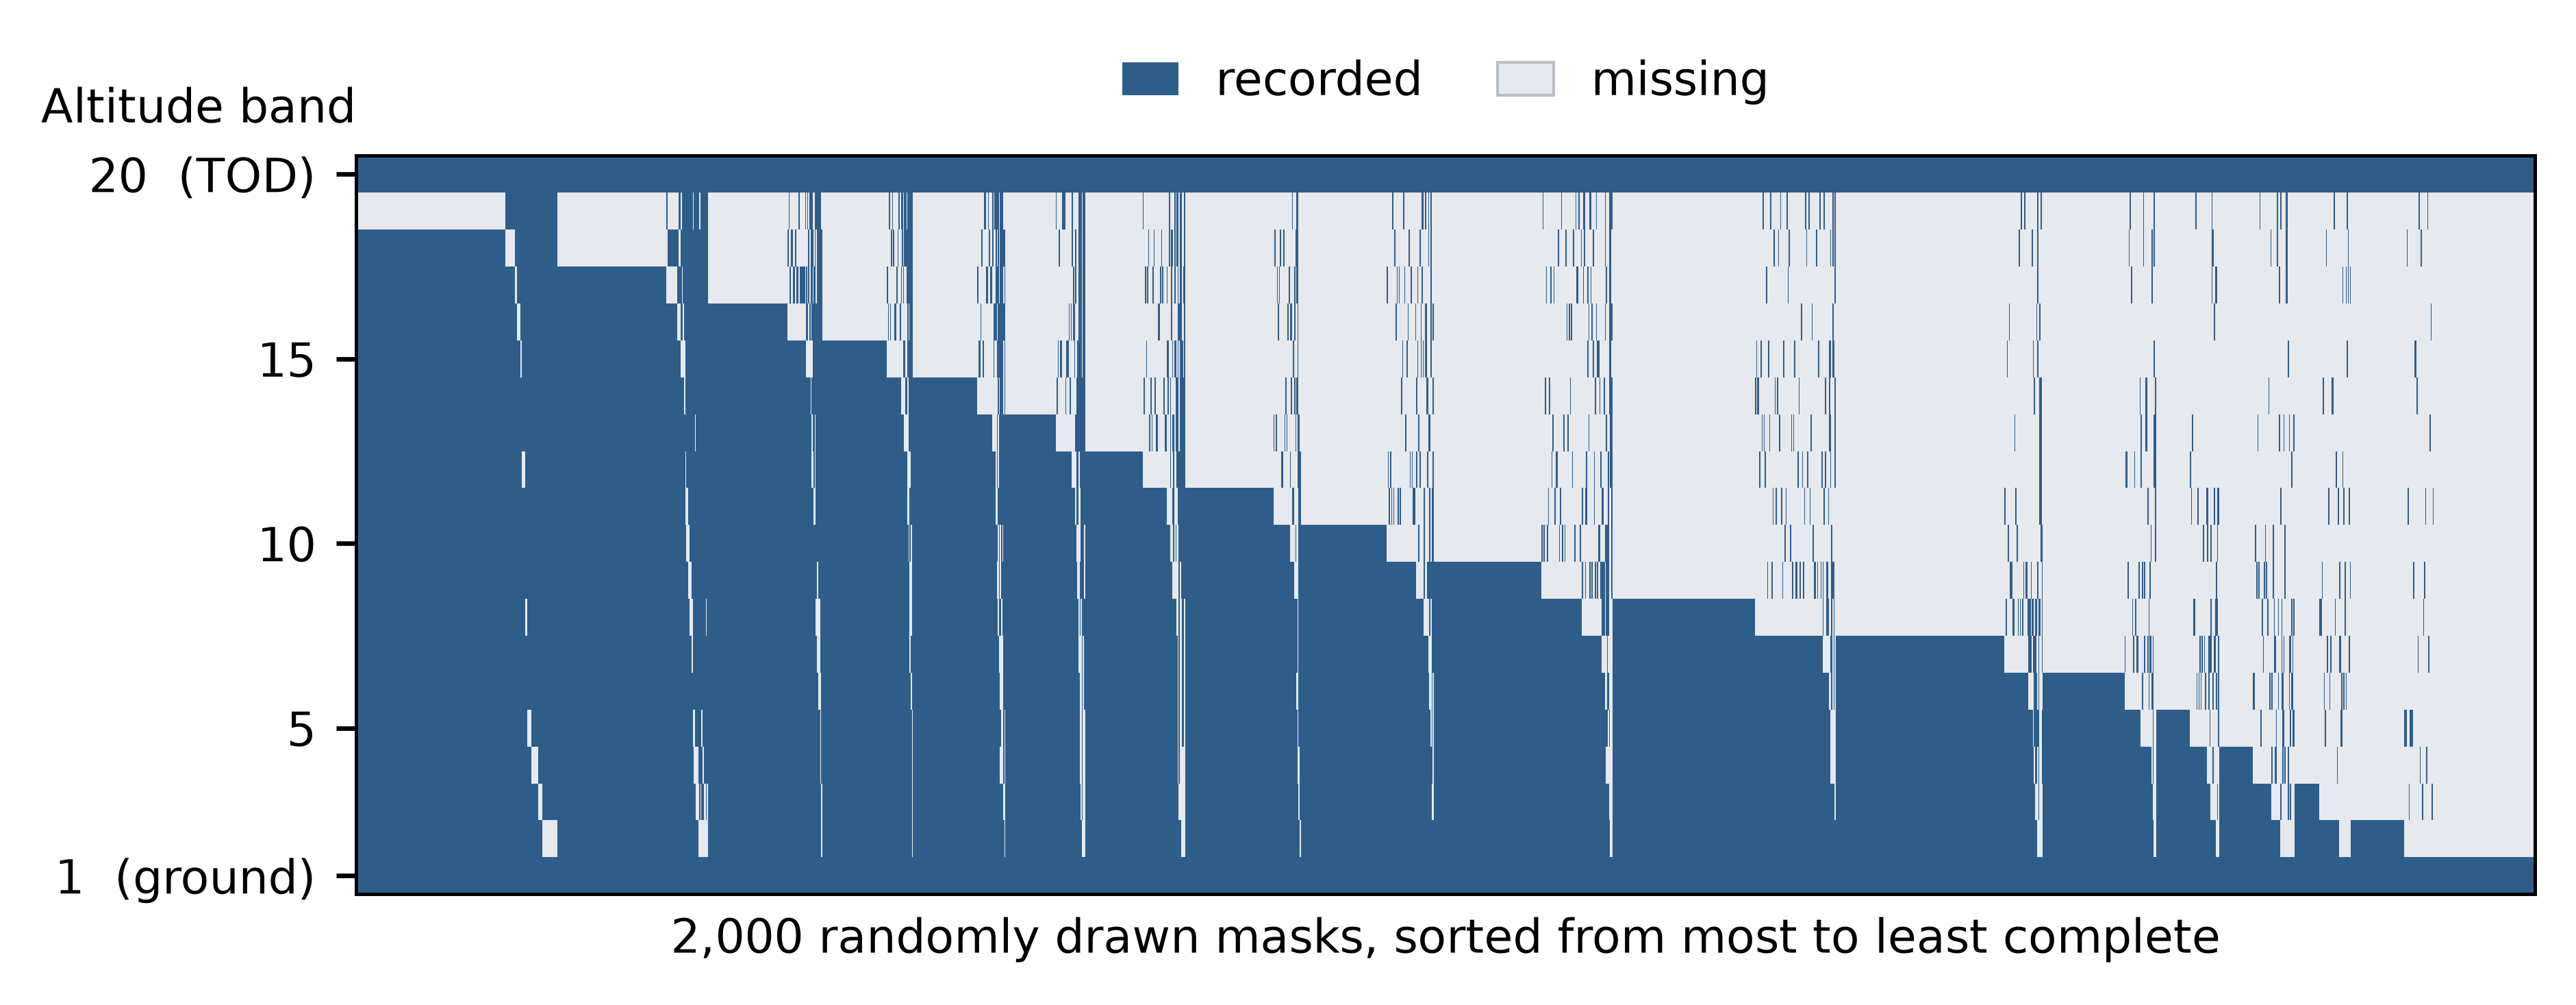
\includegraphics[width=0.8\linewidth]{figures/mask_coverage.png}
    \caption{A random sample of 2{,}000 of the 39{,}981 measured masks in the library. Each column is one incomplete descent, divided into twenty bands of equal altitude from TOD (top) to the ground (bottom). The gap typically lies just below TOD.}
    \label{fig:masks}
\end{figure}


The missing data were represented using twenty altitude bands of equal height between TOD and the ground, making descents starting at different altitudes comparable. Two types of masks were used. \emph{Measured} masks reproduce the coverage patterns observed in real ADS-B recordings. They were harvested from two months of raw recordings, separate from the test flights. Of the 79{,}513 descents considered there, each descending through at least 8{,}000~ft, about half (39{,}981 flights) had no data in at least one of the twenty altitude bands. These 39{,}981 incomplete descents form the mask library, from which one mask was drawn at random for each test flight. \emph{Synthetic} masks removed 10, 25, or 50~\% of the altitude bands, either as a contiguous block from the top or bottom of the descent, or scattered at random. They are not intended to represent realistic coverage, but to isolate the effects of the amount and location of missing data.

The measured masks show that real gaps are substantial and follow a clear pattern (Figure~\ref{fig:masks}). A typical incomplete descent contains data in only about half of the twenty altitude bands, and the missing data usually form a single continuous stretch in the upper part of the descent. Only 10~\% of the masks retain data in the band immediately below TOD, compared with 42~\% halfway down and 90~\% near the ground. A typical recording therefore captures the aircraft near TOD, loses coverage while it is farther from the receiver, and reacquires it closer to the ground station. The synthetic masks complement this by varying the amount and location of missing data independently. They can also represent truncation at the top or bottom of the descent, which the measured masks cannot because their first and last occupied bands are defined by the samples available in each recording.



\begin{table}[htbp]
    \centering
    \small
    \begin{tabular}{@{}lccc@{}}
    \toprule
    & \multicolumn{3}{c}{\textbf{MAPE [\%], loss removed from}} \\
    \cmidrule(lr){2-4}
    \thead{Synthetic masks,\\ share removed} & top & bottom & scattered \\
    \midrule
    10\,\% & 3.81 & 3.90 & 3.41 \\
    25\,\% & 4.22 & 3.95 & 3.71 \\
    50\,\% & 4.51 & 4.00 & 4.19 \\
    \midrule
    \multicolumn{2}{@{}l}{Measured mask} & \multicolumn{2}{r}{3.71} \\
    \multicolumn{2}{@{}l}{Unmasked} & \multicolumn{2}{r}{3.33} \\
    \bottomrule
    \end{tabular}
    \caption{Estimation error when part of the descent is missing, ADS-B-only features.}
    \label{tab:missing}
\end{table}

Table~\ref{tab:missing} reports the estimation error for the incomplete descents. Without applying additional masks, the flights reach 3.33~\%, close to the 3.39~\% reported in Table~\ref{tab:mapes}. The degradations can therefore be compared directly with the headline result. Applying the measured masks increases the error by only 0.38 percentage points, to 3.71~\%. The result is also stable with respect to the particular mask sample: five independent draws from the mask library gave $3.73 \pm 0.03$~\%. This robustness is consistent with the model relying substantially on aircraft-type information and MTOW, while the trajectory provides an additional correction.

The synthetic masks show how the amount and location of missing data affect the estimate separately. Removing half of the descent increases the error by 0.7--1.2 percentage points, depending on which part is removed, showing that the location of the missing data matters as much as its amount. Once a quarter or more of the descent is removed, losing the top of the descent is clearly more costly than losing the bottom: at 50~\% missing data, the error increases by 1.18 percentage points for top removal compared with 0.67 for bottom removal; at 25~\%, the corresponding increases are 0.89 and 0.62 percentage points. The upper part contains the cruise-to-descent transition and is closer in time to the mass being estimated, whereas the lower part mainly provides information related to approach speed. At 10~\% missing data, bottom removal is marginally more costly, but the difference is small. Scattered loss is the least costly of the three conditions until half of the bands are removed, as the 15~s resampling can interpolate across small gaps. With half of the bands missing, this becomes less effective because too little trajectory information remains.

One point should be kept in mind when interpreting these results. In the raw recordings, 46.4~\% of the test flights used here are already incomplete before any additional mask is applied. The unmasked condition therefore does not represent a complete descent, but the trajectory available in the original recording. The masking experiment adds a second layer of missing data on top of this naturally occurring loss.

\subsection{Limitations}
\label{sec:limitations}

Three limitations should be considered when interpreting these results. First, no independent validation data are available. Performance is evaluated using a train--test split of the same dataset rather than against independently measured TOD masses. To our knowledge, no open dataset containing measured TOD masses is currently available.

Second, the target mass is derived rather than directly observed, as discussed in Section~\ref{sec:label}. Although the target construction is reproducible, any errors in the OpenAP fuel flow model are propagated into the reference masses. The reported errors therefore measure agreement with a modelled reference rather than with the true aircraft mass.

Third, the accuracy still depends on the aircraft type and the scope of the training data. The 23 modelled types cover a large part of European airline traffic, but the dataset is not representative of global traffic and may therefore contain a regional bias. Application to aircraft from other regions or to types with different operating characteristics may introduce additional error. Section~\ref{sec:unseen} shows that the model can be applied to unfamiliar aircraft types when their MTOW and OEW are known, but the error is about 1.6 times higher than for types represented in the training data. In particular, the results for the B772 and B788 should be treated with caution, as these types showed substantially higher errors and were also strongly affected by the filtering of physically inconsistent reference masses.

\section{Conclusion}
\label{sec:conclusion}

This work presented a reusable approach for estimating aircraft mass at TOD from ADS-B data. Disclosed takeoff weights from the PRC Data Challenge 2024, propagated along each trajectory with the OpenAP fuel flow model and screened for physically impossible values, provide reference TOD masses for 464{,}633 flights. Gradient boosting models trained on openly available features reach a MAPE of 3.39~\% and an RMSE of 3{,}638~kg from ADS-B data alone, and 2.55~\% and 2{,}754~kg when weather and flight information are added.

Expressing the target as a fraction of MTOW lets the model estimate the mass of aircraft types absent from its training set, given their published MTOW and OEW: on eleven held-out types it reaches 5.56~\%, against 7.50~\% for a fixed fraction of the MTOW. The estimate is also robust to incomplete recordings: the coverage gaps observed in real ADS-B data raise the error by only 0.38 percentage points, although losing the upper part of the descent is more costly than losing the lower part. An open pipeline converts raw OpenSky state vectors into these estimates.

Three directions remain open. Independent measurements of TOD mass would allow the model to be validated against truth rather than against a modelled reference. An improved fuel flow model for the Boeing 777 and 787 families would recover the labels currently discarded by the physical check and would likely improve the estimates for these types. Finally, it remains to be tested how far the transfer to unfamiliar types extends to traffic outside Europe.


\appendix

\section{The released pipeline on independent data}
\label{app:pipeline}

Section~\ref{sec:released} describes the released pipeline; this appendix shows how it behaves on raw data. One command downloads a period of traffic from OpenSky and returns, for each arrival, the estimated mass and the time and position of TOD. An OpenSky flight list, when supplied, fills the flight-information features:

\begin{verbatim}
python estimate_tod_from_opensky.py --arrival-airport EHAM \
       --start "2026-01-01 00:00" --stop "2026-01-01 11:59:59" \
       --bounds 1,48,8,56
\end{verbatim}

\noindent Run on half a day of arrivals into Amsterdam Schiphol (1 January 2026, 00:00--12:00~UTC; 605{,}052 state vectors covering 274 aircraft-callsign pairs), the pipeline estimated the TOD mass of 194 flights, at about 0.3~s per flight on a single worker. Table~\ref{tab:funnel} accounts for the 80 rejected flights: 70 were lost to aircraft metadata, either no type in the registry (46) or no MTOW in OpenAP (24), and only ten had trajectories the method could not use.

\begin{table}[!ht]
    \centering
    \small
    \begin{tabular}{@{}lr@{}}
    \toprule
    \textbf{Stage} & \textbf{Number of flights} \\
    \midrule
    Candidate flights (\texttt{icao24} + callsign) & 274 \\
    \midrule
    Aircraft type not in the registry & $-46$ \\
    Fewer than ten samples, or never above 10{,}000~ft & $-4$ \\
    No descent phase detected & $-4$ \\
    Descent shorter than 345~s (truncated) & $-2$ \\
    No usable cruise segment & $0$ \\
    No MTOW known for the type & $-24$ \\
    \midrule
    \textbf{TOD mass estimated} & \textbf{194} \\
    \bottomrule
    \end{tabular}
    \caption{Pipeline testing on the raw OpenSky ADS-B data for half a day of Schiphol arrivals.}
    \label{tab:funnel}
\end{table}

Table~\ref{tab:sample} shows sample output, one row per flight with TOD time, position, altitude and mass.



The pipeline was also checked against the training code. Run on the raw recordings of 300 flights from the dataset, using the weather supplied with it, it reproduces exactly the nine ADS-B descent features that the training code computed for the same flights. With weather derived from \texttt{fastmeteo} instead, the weather variables agree with the dataset to within 0.6~\% on average.

\begin{table}[!ht]
    \centering
    \small
    \begin{tabular}{@{}lllcrrrr@{}}
    \toprule
    & & & \multicolumn{5}{c}{\textbf{TOD}} \\
    \cmidrule(lr){4-8}
    \textbf{callsign} & \textbf{type} & \textbf{adep} & \textbf{timestamp} & \textbf{lat} & \textbf{lon} & \textbf{alt} & \textbf{mass} \\
     & & & [UTC] & [deg] & [deg] & [ft] & [kg] \\
    \midrule
    \texttt{callsign1} & \texttt{B77L} & \texttt{OTHH} & \texttt{2026-01-01 08:43:30} & 52.06 & 7.55 & 31{,}000 & 234{,}147 \\
    \texttt{callsign2} & \texttt{A320} & \texttt{LEVC} & \texttt{2026-01-01 07:32:00} & 50.15 & 2.51 & 36{,}000 & 61{,}336 \\
    \texttt{callsign3} & \texttt{A319} & \texttt{LEMD} & \texttt{2026-01-01 09:59:30} & 50.03 & 2.38 & 38{,}000 & 54{,}858 \\
    \texttt{callsign4} & \texttt{A320} & \texttt{LEBL} & \texttt{2026-01-01 10:55:45} & 50.03 & 2.50 & 36{,}000 & 59{,}973 \\
    \texttt{callsign5} & \texttt{A320} & \texttt{LEBL} & \texttt{2026-01-01 07:54:45} & 49.11 & 3.17 & 36{,}000 & 59{,}156 \\
    \texttt{callsign6} & \texttt{A320} & \texttt{LFPG} & \texttt{2026-01-01 07:38:30} & 50.95 & 3.51 & 25{,}975 & 57{,}024 \\
    \bottomrule
    \end{tabular}
    \caption{First rows of the pipeline output for the Schiphol arrivals. The last five columns correspond to top of descent.}
    \label{tab:sample}
\end{table}


\section*{Author contributions}
\begin{itemize}
  \item Aidana Tassanbi: Conceptualization, Data Curation, Formal Analysis, Investigation, Methodology, Software, Visualization, Writing (Original Draft)
  \item Junzi Sun: Conceptualization, Data Curation, Methodology, Software, Supervision, Writing (Review and Editing)
\end{itemize}

\section*{Funding statement}
This work was performed within the NEEDED project, funded by the European Union’s Horizon Europe research and innovation programme under grant agreement no. 101095754. This publication solely reflects the authors’ view, and neither the European Union nor the funding agency can be held responsible for the information it contains.

\section*{Open data statement}
The data used in this study are available on Zenodo at \url{https://doi.org/10.5281/zenodo.23192887}.

\section*{Reproducibility statement}
\label{reproducibility}
The code used in this study, including the scripts that produce every figure and table, is publicly available at \url{https://github.com/dus42/tod_mass}.

\printbibliography

\end{document}
